\documentclass{../cheat}
\title{Digital Signal Processing}
\author{ma.mehralian}

\newenvironment{mask}
	{\renewcommand{\tabcolsep}{3pt} 
		\begin{tabular}{| >{\centering}p{10pt}| >{\centering}p{10pt} | p{10pt} | } }
	{\end{tabular}}

\begin{document}
%فیلتر ایده آل: roll off=0 فیلتر مرتبه بالا
%	• ص9: حفظ فرکانس و LTI 
%	• ص11: علی 
%	• ص20: پاسخ همگن(گذرا و مستقل از سیگنال وروری) و ویژه 
%	• ص27و28: نکته + قضیه پارسوال (تساوی انرژی در حوزه زمان و فرکانس)
%	• ص29و30: خواص تبدیل DFS
%	• ص 33: خواص تبدیل فوریه
%	• ص 38: تبدیل z=e^{j \omega}
%	• ص 42: خواص تبدیل z
%	• ص 43: قطب ها و صفرها در صفحه z
%	• ص44: رابطه پایداری با قطب (شرط پایداری وجود قطب در محدوده دایره واحد است، اگر z_i ها برابر p_i ها باشد دارای کمترین تاخیر هستیم، اگر z_i>p_i غیر علی.
%	• ص48: H(\omega)->H(z)
%	• ص61: قانون GIBSلب فرعی به اندازه 13.5dB از لب اصلی کوچکتر است.
%	• ص71: فیلترهای معروف + نکته

\begin{multicols}{3}
	\section{Discrete-Time Signals and Systems}
		\textbf{Basic sequences}
		\begin{itemize}
			\item $\delta(n)$: Unit sample sequence
				\item [-] Any discrete-time signal can be represented as a sum of scaled and shifted unit-impulses:
				$x(n)=\sum_{k=-\infty}^{\infty}x(k) \delta(n-k)$
			\item $u(n)$: Unit step sequence
			\item $x(n)=A \alpha^n$: Exponential sequences
			\item $x(n)=A \cos(\omega_0 n+ \phi)$: Sinusoidal sequences
		\end{itemize}
	
		\textbf{Discrete-time Signal}
		
		\begin{itemize}
			\item $x(n)=\sum_{k=-\infty}^{\infty}x(k) \delta(n-k)$
			%\item $y(n)=\sum_{k=-\infty}^{\infty}y(k) h(n-k)$
		\end{itemize}

		\textbf{General system}\\
		\begin{tabular}{m{0.35\columnwidth}  m{0.65\columnwidth}}
			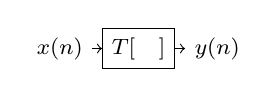
\begin{tikzpicture}[font=\footnotesize]
				\node (x)	{$x(n)$};
				\node [shape=rectangle, draw] (h)	[right of=x]	{$T[\quad]$} edge [<-] (x);
				\node (y)	[right of=h]	{$y(n)$} edge [<-] (h);
			\end{tikzpicture} &
				system response \hfill $x(n) \rightarrow y(n)$ \hspace{15pt} \null \newline
				unit sample response \hfill $\delta(n) \rightarrow h(n)$ \hspace{15pt} \null\\
		\end{tabular}

		\textbf{Linear Time-Invariant (LTI or LSI) Systems}\\
		if $x_1(n) \rightarrow y_1(n)$ and  $x_2(n) \rightarrow y_2(n)$
		\begin{itemize}[nolistsep, leftmargin=1em]
			\item \textbf{linearity}:	$T[ax_1(n) + bx_2(n)] = ay_1(n) + by_2(n)$
			\item \textbf{time-invariant}:	$T[x(n-n_0)] = y(n-n_0)$
			\item A linear system is completely characterised by its impulse response
		\end{itemize}

		
		\textbf{Convolution Sum}
		\begin{itemize}
			\item $y(n)=\sum_{k=-\infty}^{\infty}x(k) h(n-k)$
			\item $y(n) = x(n) \ast h(n) = h(n) \ast x(n)$
			\item $x(n) \ast (h_1(n) + h_2(n))=x(n) \ast h_1(n) + x(n) \ast h_2(n)$
			\item $(x(n) \ast h_1(n)) \ast h_2(n) = x(n) \ast (h_1(n) \ast h_2(n))$
		\end{itemize}
		
		\textbf{Stability}
		\begin{itemize}
			\item General: every bounded input sequence produces a bounded output sequence.
				%If $x(n)$ bounded ie $|x(n)|<\infty$ all $n$ then $y(n)$ bounded ie $|y(n)|<\infty$ all $n$
			\item LSI: $\sum_{k=-\infty}^{\infty} |h(n)| < \infty$
			\item e.g., unstable: $h(n)=2^n u(n)$\hfill stable: $h(n)=\frac{1}{2}^n u(n)$
		\end{itemize}
		
		\textbf{Causality}
		\begin{itemize}
			\item General: $y(n)$ for $n=n_i$ depends on $x(n)$ only for $n \leq n_i$
			\item LSI: $h(n)=0 \quad n<0$
			\item e.g., non-causal stable: $h(n)=2^n u(-n)$
		\end{itemize}
		
		\textbf{System impulse response}(??)
		\begin{itemize}
			\item Finite-duration impulse response (FIR) system: The impulse response has only a finite number of nonzero samples.
			\item Infinite-duration impulse response (IIR) system: The impulse response is infinitive in duration.
			\item FIR systems always are stable, if each of $h[n]$ values is finite in magnitude.
‰			\item IIR systems can be stable
		\end{itemize}
		
		\textbf{Difference Equation}
		\begin{itemize}
			\item An important class of LTI systems
			\item $N^{th}$ order: $\sum_{k=0}^{N} a_k y(n-k) = \sum_{r=0}^{M} b_r x(n-r)$
			\item $1^{st}$ order: $y(n)+ay(n-1)=x(n)$
		\end{itemize}
		
		\textbf{Frequency Response of LSI system}
		\begin{itemize}
			\item $y(n)=\sum_{k=-\infty}^{+\infty}	h(k) x(n-k)$ \quad let $x(n)=e^{j \omega n}$\\
				$y(n)=\sum_{k=-\infty}^{\infty} h(k) e^{j\omega (n-k)}$\\
				$y(n)=e^{j\omega n}\sum_{k=-\infty}^{\infty} h(k) e^{- j\omega k}$\\
				$y(n)=H(e^{j\omega})e^{j\omega n}$
			\item The frequency response of discrete-time LTI systems is always a periodic function of the frequency variable $\omega$ with period $2\pi$. Only specify over the interval $-\pi < \omega <\pi$
		\end{itemize}
		
		
		expressing a signal in terms of sinusoids will lead us to the Fourier transform
		
		$g[x] = e^{i\omega x} \ast h[x]$
		
		$A e^{i \omega x}=A \cos( \omega x)+i A\sin( \omega x)$
		
		\begin{align*}
				g[x]&=e^{i\omega x} \star h[x] \nonumber\\
				&=\sum_{k=-\infty}^{\infty}h[k] e^{i\omega(x-k)} \nonumber\\
				&=e^{i\omega x}\sum_{k=-\infty}^{\infty}h[k] e^{-i\omega k}
		\end{align*}
		
% You can even have references
\vspace{5mm}
\rule{0.3\linewidth}{0.25pt}
\scriptsize

\textbf{References:}
\begin{itemize}[leftmargin=2em]
	\item [{[1]}] Discrete Time Signal Processing 2nd Ed, by Alan V. Oppenheim, Ronald W. Schafer
\end{itemize}
Made by \href{http://webpages.iust.ac.ir/mehralian/}{ma.mehralian} using \LaTeX
\end{multicols}

\end{document}